\documentclass[12pt]{report}
\usepackage[utf8]{inputenc}
\usepackage{amsmath,mathpazo,siunitx,xparse,tikz,enumitem,fancyhdr,pgfplots}
\usepackage{geometry}[1in]
\usepackage[document]{ragged2e}
\usepackage{tabularx}
\usepackage{tabulary}
\usepackage{pgfplotstable}
\usepackage{longtable}
\usepackage{booktabs}
\usepackage{xtab}
\usepackage{paracol}
\usepackage{array}
\usepackage{multicol}
\usepackage{paracol}
\usetikzlibrary{patterns}

\makeatletter
\newcommand{\pgfplotsdrawaxis}{\pgfplots@draw@axis}
\makeatother
%%Needed to properly display graphs
\pgfplotsset{only axis on top/.style={axis on top=false, after end axis/.code={
             \pgfplotsset{axis line style=opaque, ticklabel style=opaque, tick style=opaque,
                          grid=none}\pgfplotsdrawaxis}},compat=1.9,width=5.5in}
%\pgfplotsset{width=10cm,compat=1.9}

\pagestyle{fancy}
\fancyhf{}
\lhead{Steven Glasford}
\chead{Homework 3}
\rhead{Page \thepage}

\title{Homework 3}
\author{Steven Glasford}
\date{\parbox{\linewidth}{\centering%
    %%Adds the last compiled date
    \today\endgraf\medskip
    Math-451-M001}}

%%Creates a new symbol for plus and minus together
\newcommand{\rpm}{\sbox0{$1$}\sbox2{$\scriptstyle\pm$}
  \raise\dimexpr(\ht0-\ht2)/2\relax\box2 }

%%Creates a nice format for displaying the steps taken  
\newlist{steps}{enumerate}{1}
\setlist[steps, 1]{label = Step \arabic*:}

\ExplSyntaxOn
%%new command to round numbers
\newcommand*{\prlen}[1]{%
   % round to 1 digit:
    \pgfmathparse{round(10)/10.0}%
    %\pgfkeys{/pgf/number format/precision=1}
    %\pgfmathresult
    \pgfmathprintnumber[fixed, precision=2]{\pgfmathresult}
}
\ExplSyntaxOff

\newcommand{\drawge}{-- (rel axis cs:1,0) -- (rel axis cs:1,1) -- (rel axis cs:0,1) \closedcycle}
\newcommand{\drawle}{-- (rel axis cs:1,1) -- (rel axis cs:1,0) -- (rel axis cs:0,0) \closedcycle}


\begin{document}
%% adds the title to the document
\maketitle
%% adds the table of contents to the document
\tableofcontents

%%Add everything about the first problem here
\chapter{War}

\section{Problem Statement}
Two armies are to engage in battle. The red army enjoys a three-to-one numerical superiority, but the blue army is better trained and better equipped. Let $R$ and $B$ denote the force levels of red and blue forces. The Lanchester model of combat states that $$R'=-aB-bRB$$ $$B'=-cR-dRB,$$ where the first term accounts for direct fire (aimed at a specific target) and the second term accounts for attrition due to area fire (e.g., artillery). We are assuming that weapon effectiveness is higher for blue than for red; i.e., $a>c$ and $b>d$. But what kind of edge in weapon effectiveness would be necessary to counteract a $3:1$ numerical superiority?

\begin{enumerate}[label=(\alph*),ref=(\alph*)]
    
    \item \label{1} Assuming that $a=\lambda c$ and $b=\lambda d$ for some $\lambda > 1$, determine the approximate lower bound on $\lambda$ necessary for blue to win the war. Use the five-step method, and model as a dynamical system.
    
    \item In part \ref{1} you assumed red had a $n:1$ numerical superiority. Discuss the sensitivity of your results in part \ref{1} to the parameter $n \in (2, 5)$.
    
\end{enumerate}

\section{Presentation of the Model}


    \begin{tabularx}{\linewidth}{ l X}
        
         \textbf{Variables:}&  
         
         
         %\begin{tabular}[t]{l@{\hspace{3mm}}l@{\hspace{3mm}}p{6in}}
         \begin{tabulary}{\linewidth}[t]{LLL}
              $R'$&$=$ & Change in the size of the Red Army.\\
              $B'$&$=$ & Change in the size of the Blue Army.\\
              $R$&$=$& The current size of the Red Army.\\
              $B$&$=$& The current size of the Blue Army.\\
              $a$&$=$ & Weapon effectiveness from direct fire from the Blue Army.\\
              $c$&$=$ & Weapon effectiveness from direct fire from the Red Army.\\
              $b$&$=$& Weapon effectiveness from attrition from the Blue Army.\\
              $d$&$=$& Weapon effectiveness from attrition from the Red Army.\\
              $\lambda$&$=$& Level of weapons sophistication for the Blue Army.\\
              $n$&$=$& The factor of numerical superiority for the Red Army.\\
              $t$&$=$& Time.\\ 
              $R_0$&$=$& Initial size of the Red Army.\\
              $B_0$&$=$& Initial size of the Blue Army.\\
              $R_f$&$=$& Final size of the Red Army.\\
              $B_f$&$=$& Final size of the Blue Army.\\
              
         \end{tabulary}
        
         \\
        
         \textbf{Assumptions:}&
         
         \begin{tabulary}{\linewidth}[t]{LLL}
              $R'$&$=$ & $-aB-bRB$\\
              $B'$&$=$&$-cR-dRB$\\
              $a$&$>$&$c$\\
              $b$&$>$&$d$\\
              $a$&$=$&$\lambda c$\\
              $b$&$=$&$\lambda d$\\
              $\lambda$&$>$&1\\
              $R_0$&$=$&$nB_0$\\
              $n$&$=$&3\\
              $B_0$&$>$&0\\
              $R_0$&$>$&0\\
              $R_f$&$>$&0\\
              $B_f$&$>$&0\\
              $c$&$=$&$.05$\\
              $d$&$=$&$.005$\\
              
         \end{tabulary}
         \\
         
         \textbf{Objective:} & Determine the lower bound on $\lambda$ necessary for blue to win the war.\\
         
    \end{tabularx}

\section{Solving the Model}
\hspace{5mm} To solve this model we shall first put $R'$ and $B'$ into a ratio, this ratio will determine which side is dying faster. A ratio factor greater than 1 indicates one army is doing better than the other army, and the a ratio less than 1 indicates one army dying faster than the other, and a ratio equal to 1 indicates that the death rate on both sides is equal.

\hspace{5mm} It doesn't really mater which equation goes on top, so we will This gives us an equation that looks like the following:

$$\dfrac{B'}{R'} = \dfrac{-cR-dRB}{-cR-dRB}$$

If this ratio is greater than 1, then the Blue forces are winning, if it is less than 1, then the Red forces are winning. This equation is also a nonlinear equation so we are going to solve for both $B'$ and $R'$ individually using the mathematical software Maple. 

When we solve get a statement that $B=B$ and a very long and complicated function for $R$. We don't really care if $B$ is equal to itself as this doesn't tell us any new information, but the complicated equation for $R$ is a step in the right direction. The actual function produced by Maple as the Function for $R$ is:

$$R=e^{-\dfrac{1}{10\lambda}\left(10\cdot LambertW\left(\dfrac{B^{\left(\dfrac{1}{\lambda}\right)}e^{\left(\dfrac{B}{10\lambda}+\dfrac{R_0}{10\lambda}\right)}}{10}\right)\lambda-10\ln{(B)}-B-R_0\right)}$$
\bigskip
Which is very confusing to look at. 

Now we are going to make a couple further assumptions about this equation. We will assume the battle has been completed and one side one the battle. This means all of the $R$ values will indicate the final Red soldier counts ($R_f$) and all instances of of $B$ will indicate the final Blue soldier counts ($B_f$), $R_0$ is a constant and indicates the initial size of the Red army, and finally $LambertW$ is a Maple special function.

\bigskip

We can replace $R_0$ with $R_0=nB_0$, where $n=3$.

This would produce an equation like:

$$R_f=e^{-\dfrac{1}{10\lambda}\left(10\cdot LambertW\left(\dfrac{B_f^{\left(\dfrac{1}{\lambda}\right)}e^{\left(\dfrac{B_f}{10\lambda}+\dfrac{3B_0}{10\lambda}\right)}}{10}\right)\lambda-10\ln{(B_f)}-B_f-3B_0\right)}$$

\medskip

Now we want to find a $\lambda$ value where $B_f$ will indicate an obvious victory for the Blue team. The most obvious indication of a Blue win would be when $R_f$ is zero and $B_f$ is nothing greater than 1, but if this where the case $\lambda$ literally doesn't equal anything. So we must find a different case where Blue has an obvious win.

\medskip

We shall now assume that only \emph{one} person does not die in battle from the Red army, and the Blue team survives by a large margin (this one person could presumably be taken prisoner of war by the Blue army, meaning the Blue army has still won the battle).

\smallskip

This changes our assumptions for $R_f$ to:
$$R_f=1$$

We now try to find a solution for $\lambda$ with the new $R_f$ value in the function from above using Maple again, which finds that $$\lambda = 10\ln{(B_0)}+B_0+3B_f$$

We are told that $\lambda > 1$, this means that $$1 < 10\ln{(B_0)}+B_0+3B_f$$ must also be true.

Solving for $B$ gives the inequality: $$B_f>\dfrac{-10\ln{(B_0)}+B_0-1}{3}$$
Whenever this is true then $\lambda$ is true, which means this inequality is the boundary of $\lambda$. Figure \ref{fig:inequality} is the graphed out inequality of the this function.

\smallskip

  \begin{figure}[th] 
    \centering 
    \label{fig:inequality} 
    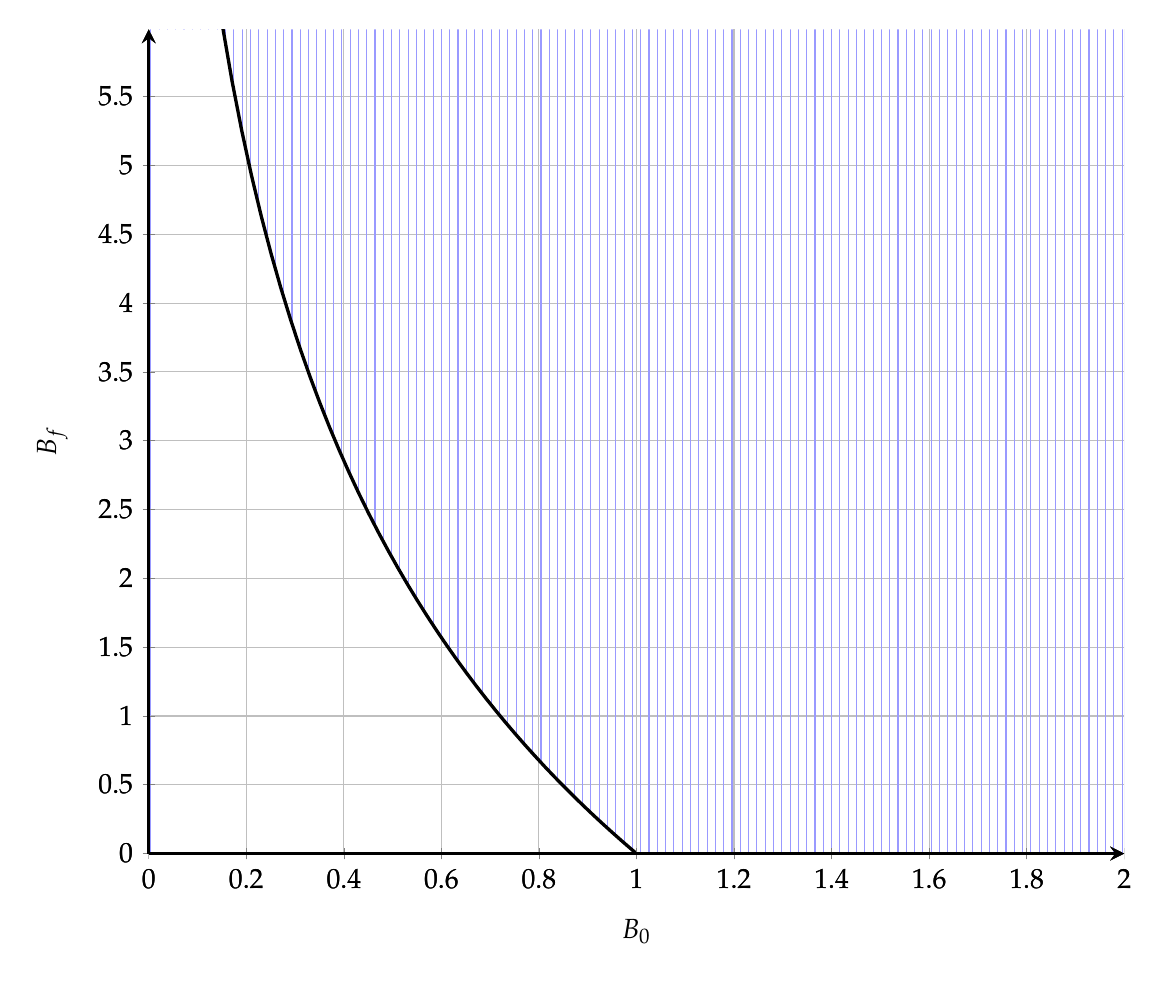
\begin{tikzpicture} 
      \begin{axis}[only axis on top,
        axis line style=very thick, 
        axis x line=bottom, 
        axis y line=left, 
         ymin=0,ymax=5.99,xmin=0,xmax=2, 
         xlabel=$B_0$, ylabel=$B_f$,grid=major 
      ] 
        \addplot [draw=none, pattern=vertical lines, pattern color=blue!40, domain=-10:4,samples = 1000]
                 {(-10*ln(x)+x-1)/3} \drawge; 

        \addplot[very thick, domain=-10:10, samples = 1000] {(-10*ln(x)+x-1)/3}; 

      \end{axis} 
    \end{tikzpicture} 
    \caption{Plot of $B_f>\dfrac{-10\ln{(B_0)}+B_0-1}{3}$} 
  \end{figure} 
  
  \section{Sensitivity Analysis}
  In the equations from above we assumed that red had an $3:1$ numerical superiority, we shall now do a sensitivity analysis for when $n:1$.
 
  \bigskip 
  
  If we replace $R_0=3B_0$ with $R_0=nB_0$ we end and doing all of the calculations from above to get an equation for $\lambda$ we end up getting: $$\lambda=10\ln{(B_0)}+B_0+nB_f$$
  
  We shall find the sensitivity of $\lambda$ to $n$ when $n \in{(2,5)}$. To do this we shall find $S(n,\lambda)$. Since $S(n,\lambda)$ typically equals $$S(n,\lambda)=\dfrac{dn}{d\lambda}\cdot \dfrac{\lambda}{n}$$ and $n$ is not a function, but rather a series of intervals, we shall use an approximation of of $S(n,\lambda)$, in this case we will approximate it by: $$S(n,\lambda)\approx \dfrac{\Delta n}{\Delta \lambda}\cdot \dfrac{\lambda}{n},$$ and since we are given two different new $n$ values we shall perform this operation twice and average the two sensitivities. 
  
  \bigskip
  
  For the first one, where $n=2$, we get $$S(n,\lambda)\approx\dfrac{3-2}{(10\ln{(B_0)}+B_0+3B_f)-(10\ln{(B_0)}+B_0+2B_f)}\cdot \dfrac{10\ln{(B_0)}+B_0+2B_f}{3}$$ which simplifies to 
  $$S(n,\lambda)\approx \dfrac{10\ln{(B_0)}+B_0+2B_f}{2B_f}$$ 
  where $B_0$ and $B_f$ are held as constants.
  
  \bigskip 
  
  Next we find the sensitivity at the next element, when $n=5$. So $$S(n,\lambda)\approx\dfrac{3-5}{(10\ln{(B_0)}+B_0+3B_f)-(10\ln{(B_0)}+B_0+5B_f)}\cdot \dfrac{10\ln{(B_0)}+B_0+5B_f}{5}$$
  which simplifies to
  $$S(n,\lambda)\approx \dfrac{10\ln{(B_0)}+B_0+5B_f}{5B_f}$$
  again, where $B_0$ and $B_f$ are held as constants.
  
  \bigskip
  
  Now we take the average of these two sensitivities:
  $$\overline{S(n,\lambda)}=\dfrac{\dfrac{10\ln{(B_0)}+B_0+5B_f}{5B_f} + \dfrac{10\ln{(B_0)}+B_0+2B_f}{2B_f}}{2}$$
  
  which simplifies to:
    $$\overline{S(n,\lambda)}=\dfrac{70\ln{(B_0)}+7B_0+20B_f}{20B_f}  $$
    
    \bigskip
    
    Figure \ref{fig:sensitivity} is the plotted sensitivity, and Figure \ref{fig:profile} is the profile view of sensitivity plot at $S(n,\lambda)=0$

\begin{figure}[th] 
    \centering 
    \label{fig:sensitivity} 
    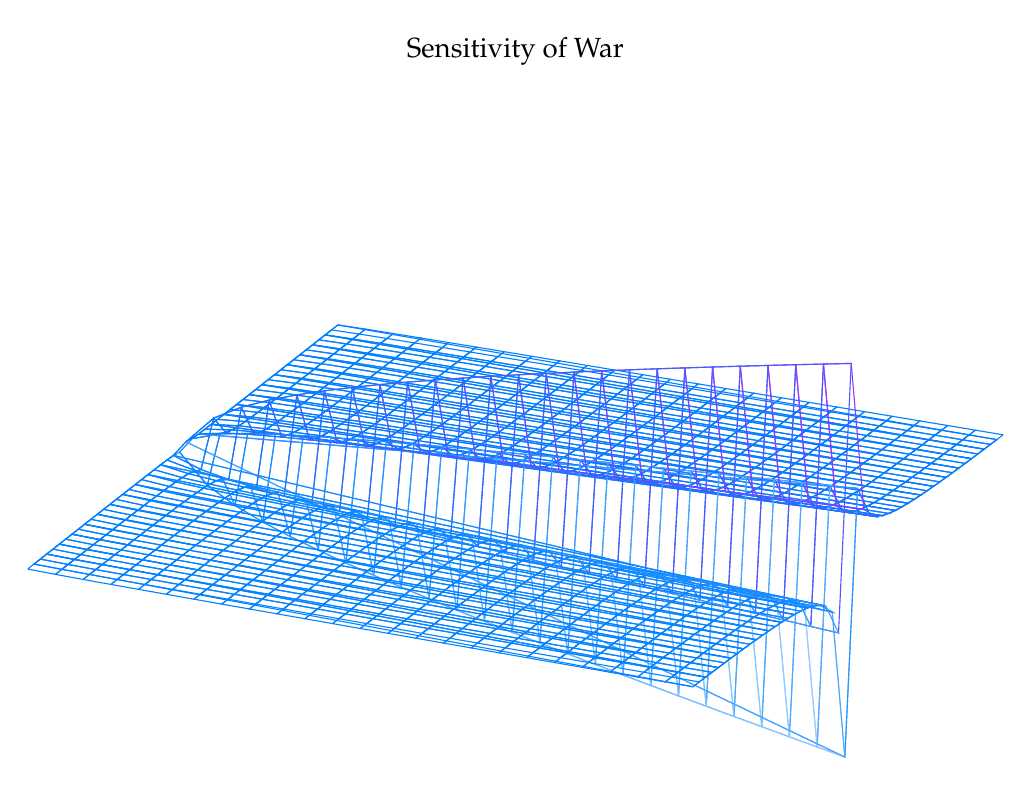
\begin{tikzpicture} 
      \begin{axis}[
      title = {Sensitivity of War},
      hide axis,
      colormap/cool,
      ] 
        \addplot3 [
            mesh,
            samples=50,
            domain =-50:50,
        ]
        {(10*ln(x)+x+5*y)/(5*y}; 

         

      \end{axis} 
    \end{tikzpicture} 
    \caption{Sensitivity plot, the center of the ridge is at zero} 
  \end{figure}
  
  \begin{figure}[th] 
    \centering 
    \label{fig:profile} 
    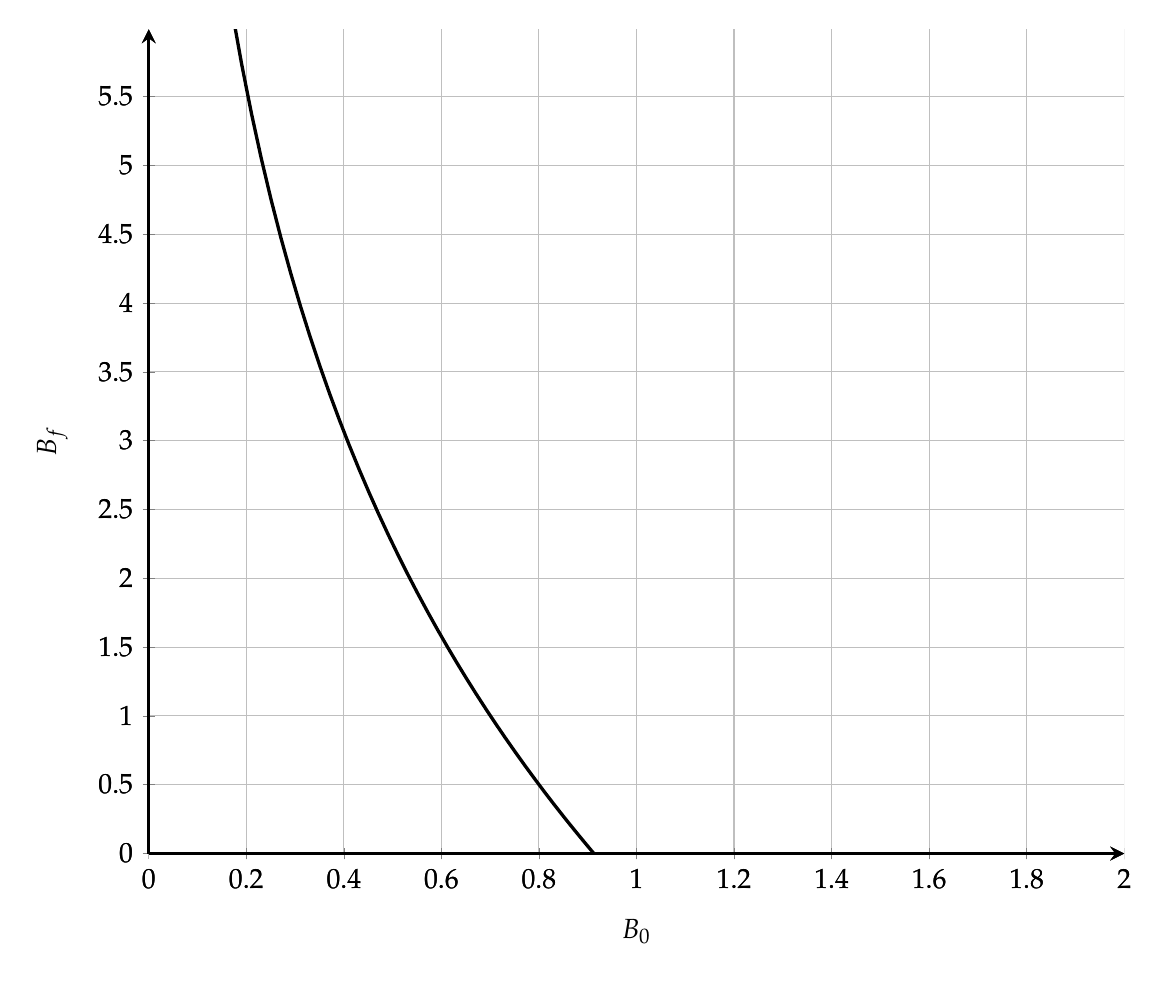
\begin{tikzpicture} 
      \begin{axis}[only axis on top,
        axis line style=very thick, 
        axis x line=bottom, 
        axis y line=left, 
         ymin=0,ymax=5.99,xmin=0,xmax=2, 
         xlabel=$B_0$, ylabel=$B_f$,grid=major 
      ] 

        \addplot[very thick, domain=-10:10, samples = 1000] {-(7*ln(x)/2)-(7*x/20)}; 

      \end{axis} 
    \end{tikzpicture} 
    \caption{Profile view of the sensitivity plot} 
  \end{figure} 

%The second assigned problem
\chapter{Disease}

\section{Problem Statement}
A population of 100,000 members is subject to a disease that is seldom fatal and leaves the victim immune to future infections by this disease. Infection can only occur when a susceptible person comes in contact with an infectious person. The infection period lasts approximately three weeks. Last week, there were 18 new cases of the disease reported. This week, there were 40 new cases. It is estimated that 30\% of the population is immune due to previous exposure.

\begin{enumerate}[label=(\alph*),ref=(\alph*)]
    \item \label{2} What is the eventual number of people who will become infected? Use the five-step method, and model as a discrete-time dynamical system.
    \item Estimate the maximum number of new cases in any one week.
    \item Conduct a sensitivity analysis to investigate the effect of any assumptions you made in part \ref{2} that were not supported by hard data.
    \item Perform a sensitivity analysis for the number of cases (18) reported last week. It is thought by some that in early weeks the epidemic might be under-reported.
\end{enumerate}

\section{Presentation of the Model}

\begin{tabularx}{\linewidth}{ l X}
        
         \textbf{Variables:}&  
         
         
         %\begin{tabular}[t]{l@{\hspace{3mm}}l@{\hspace{3mm}}p{6in}}
         \begin{tabulary}{\linewidth}[t]{LLL}
            $S$&$=$& The number of people susceptible to the pathogen.\\
            $I$&$=$& The number of infected people.\\
            $R$&$=$& The number of recovered and immune people.\\
            $P$&$=$& The total number of people in the population.\\
            $t$&$=$& Time.\\
            $S'$&$=$& The change in the number of susceptible people.\\
            $I'$&$=$& The change in the number of infected people.\\
            $R'$&$=$& The change in the number of recovered people.\\
            $N$&$=$& Total number of people who have been infected and now are immune to the disease\\
              
         \end{tabulary}
        
        \\
        
         \textbf{Assumptions:}&
         
         \begin{tabulary}{\linewidth}[t]{LLL}
              && No one dies and no one is born with in the time the disease is around;\\
              && AND once a person has recovered from the disease, he or she will be infinitely immune to the disease;\\
              && AND the number of people infected changes in intervals (this should be treated as a discrete model);\\
              && AND after three weeks of having the disease, the person is recovered from the disease and therefore, now immune to the disease; \\
              $P$&$=$&$S+I+R$\\
              $P$&$=$&100,000\\
              $I_0$&$=$&0\\
              $I_1$&$=$&18\\
              $I_2$&$=$&40\\
              $R_0$&$=$&$.3P$\\
              $N$&$=$&$R+I$\\
              $S'$&$=$&$S_n-S_{n-1}$\\
              $I'$&$=$&$I_n-I_{n-1}$\\
              $R'$&$=$&$R_n-R_{n-1}$\\
              
         \end{tabulary}
         \\
         
         \textbf{Objective:} & Determine the number of people who will eventually become infected ($N$).\\
         
    \end{tabularx}

\section{Solving the Model}
We must now determine the equations we should use for $S_n$, $I_n$, $R_n$, as well as for $S'$, $I'$, and $R'$.

\bigskip

Since after three weeks of having the disease, a person is fully recovered and immune to the disease. This would make 
\begin{align}
    R' &= I_{n-3} \label{eq:4}
\end{align}
where $n$ is an iteration of the discrete system. This would also make 
\begin{align}
    I' &= I_{n-2}-I_{n-3} \label{eq:5}
\end{align}

Now we need to find an equation for $S'$. Before that we must use some of the assumptions we made in the beginning, in particular, we know there are no births or deaths in the population so the we can reason that 
\begin{align}
    P' &= 0 \label{eq:6}
\end{align}
and since 
\begin{align}
    P &= S+I+R \label{eq:7}
\end{align}    
is true then 
\begin{align}
    P' &= S'+I'+R' \label{eq:8}
\end{align}
should also be true. And using the information from (\ref{eq:6}) we can rewrite this function as 
\begin{align}
    0 &= S'+I'+R' \label{eq:9}
\end{align}

We can then solve for $S'$ to get 

\begin{align}
    S' &= -I'-R' \label{eq:10}
\end{align}

But our model doesn't really care for the the change in the variables, we care about the total number of infected individuals and the total number of people who have ever had this disease. To do this we need to find $S_n$, $I_n$, and $R_n$. To find these values we use the following information from our list of assumptions: 
\begin{align}
    S' &= S_n-S_{n-1} \label{eq:1}\\
    I' &= I_n-I_{n-1} \label{eq:2}\\
    R' &= R_n-R_{n-1} \label{eq:3}                            
\end{align}

Using the equations (\ref{eq:1}), (\ref{eq:2}), and (\ref{eq:3}) we get the following new functions:
\begin{align}
    S_n-S_{n-1} &= -(I_{n-2}-I_{n-3})-(I_{n-3}) \label{eq:11}\\
    I_n-I_{n-1} &= I_{n-2}-I_{n-3} \label{eq:12}\\
    R_n-R_{n-1} &= I_{n-3} \label{eq:13}
\end{align}

If we solve (\ref{eq:14}) for $S_n$ we get
\begin{align}
    S_n &= S_{n-1}+I_{n-2} \label{eq:14}
\end{align}

If we solve (\ref{eq:15}) for $I_n$ we get
\begin{align}
    I_n &= I_{n-1}+I_{n-2}-I_{n-3} \label{eq:15}
\end{align}

And if we solve (\ref{eq:16}) for $R_n$ we get
\begin{align}
    R_n &= R_{n-1}+I_{n-3} \label{eq:16}
\end{align}

We can now find a relation for $N$ from equations (\ref{eq:14}), (\ref{eq:15}), and (\ref{eq:16}). From our list of assumptions we know 
\begin{align}
    N &= R+I \label{eq:17}\\
    N_n &= R_n+I_n \label{eq:18}
\end{align}

Where (\ref{eq:18}) is the discrete version of (\ref{eq:17}). We then substitute $I_n$ and $R_n$ from (\ref{eq:15}) and (\ref{eq:16}) into equation \ref{eq:18} to get
\begin{align}
    N_n &= R_{n-1}+I_{n-3}+I_{n-1}+I_{n-2}-I_{n-3} \nonumber\\
        &= R_{n-1}+I_{n-1}+I_{n-2} \label{eq:20}
\end{align}

Now we can solve our objective. Notice how this is a recursive function so we will use a computer to do the computations and we will save the data into the table on the next page.


%\begin{tabular}{| c | c | c | c | c |}\hline%
%\bfseries S & \bfseries I & \bfseries R & \bfseries N & \bfseries Week
%\csvreader[head to column names]{data.csv}{} % 
%{\\\hline\csvcoli & \csvcolii & \csvcoliii & \csvcoliiii & \csvcoliiiii} % 
%\\\hline
%\caption{Raw Data from our recursive Relations}\label{tab:stats}
%\end{tabular}


\pgfplotstableset{
begin table=\begin{longtable},
end table=\end{longtable},
every head row/.style={before row=\toprule, after row=\midrule\endhead}
}

\pgfplotstabletypeset[col sep=comma,
    columns/S/.style=
        {column type/.add={>{\small}}{}},
    columns/I/.style=
        {column type/.add={>{\small}}{}},
    columns/R/.style=
        {column type/.add={>{\small}}{}},
    columns/N/.style=
        {column type/.add={>{\small}}{}},
    columns/New/.style=
        {column type/.add={>{\small}}{}},
    columns/Week/.style=
        {column type/.add={>{\small}}{}},
    ]{data.csv}

We see that eventually the number of susceptible people becomes zero (see also figure \ref{susceptible} for a graphical version for the number of susceptible people). So eventually every single person has once been infected by the disease. So by the $84^{th}$ week all 100,000 people will have once been infected by the disease.

\bigskip

We can also see from the ``New" column that the number of new is constantly increasing, right up until the very last day of the disease, notice that the disease actually exists for one more week, but that the there is not enough susceptible people to infect so the next week the number of susceptible people is zero the next week. So the maximum number of new cases in one week is 1,658.

\bigskip

\section{Sensitivity Analysis}
We made no further assumptions or variables so a sensitivity analysis on those variables is not necessary.
But according to recent reports, the number of cases initially reported (18) may have been underreported so we shall perform a sensitivity analysis on the number of initial cases reported. We shall take two cases, each with 3 subcases.

\bigskip



We shall then try some different cases, but we will not be displaying any more giant tables like the one already seen, instead we will just display the quick stats (a.k.a. the last line of the table similar to the table already seen).

\begin{itemize}
    \item \emph{\textbf{Case 1: } Cases reported at week -1 = 20}
    
    \begin{tabular}{|c|c|c|c|c|c|}
        \hline
        S&I&R&N&New&Week\\
        \hline
        240&	1700&	98060&	99760&	1660&	83\\

        \hline
    \end{tabular}
    
    \item \emph{\textbf{Case 2: } Cases reported at week -1 = 22}
    
    \begin{tabular}{|c|c|c|c|c|c|}
        \hline
        S&I&R&N&New&Week\\
        \hline
        156&	1702&	98142&	99844&	1662&	83\\


        \hline
    \end{tabular}
    
    \item \emph{\textbf{Case 3: } Cases reported at week -1 = 24}
    
    \begin{tabular}{|c|c|c|c|c|c|}
        \hline
        S&I&R&N&New&Week\\
        \hline
        72&	1704&	98224&	99928&	1664&	83\\


        \hline
    \end{tabular}
    
\end{itemize}


\begin{figure}[p]
\begin{center}
    \begin{tikzpicture}
        \begin{axis}[
                title = {Susceptible People}
                axis lines = left,
                xlabel = {Weeks},
                ylabel = {Number of People},
                scaled ticks = false,
                tick label style = {/pgf/number format/fixed}
            ]
            \addplot table [x=Week, y=S, col     sep=comma] {data.csv};
        \end{axis}
    \end{tikzpicture}
    \label{susceptible}
    \caption{Plot of the Number People Susceptible to the Disease}
\end{center}
\end{figure}

\begin{figure}[p]
\begin{center}
    \begin{tikzpicture}
        \begin{axis}[
                title = {New Cases}
                axis lines = left,
                xlabel = {Weeks},
                ylabel = {Number of People},
                scaled ticks = false,
                tick label style = {/pgf/number format/fixed}
            ]
            \addplot table [x=Week, y=New, col     sep=comma] {data.csv};
        \end{axis}
    \end{tikzpicture}
    \label{susceptible}
    \caption{Plot of the Number of New Case per Week}
\end{center}
\end{figure}

\begin{figure}[p]
\begin{center}
    \begin{tikzpicture}
        \begin{axis}[
                title = Infected People
                axis lines = left,
                xlabel = {Weeks},
                ylabel = {Number of People},
                scaled ticks = false,
                tick label style = {/pgf/number format/fixed}
            ]
            \addplot table [x=Week, y=I, col     sep=comma] {data.csv};
        \end{axis}
    \end{tikzpicture}
    \label{infected}
    \caption{Plot of the Number People Currently Infected by the Disease}
\end{center}
\end{figure}

\begin{figure}[p]
\begin{center}
    \begin{tikzpicture}
        \begin{axis}[
                title = {Recovered People},
                axis lines = left,
                xlabel = {Weeks},
                ylabel = {Number of People},
                scaled ticks = false,
                tick label style = {/pgf/number format/fixed}
            ]
            \addplot table [x=Week, y=R, col     sep=comma] {data.csv};
        \end{axis}
    \end{tikzpicture}
    \label{recovered}
    \caption{Plot of the Number People who have Recovered from the Disease}
\end{center}
\end{figure}

\begin{figure}[p]
\begin{center}
    \begin{tikzpicture}
        \begin{axis}[
                title = {People who have had the Disease},
                axis lines = left,
                xlabel = {Weeks},
                ylabel = {Number of People},
                scaled ticks = false,
                tick label style = {/pgf/number format/fixed}
            ]
            \addplot table [x=Week, y=N, col     sep=comma] {data.csv};
        \end{axis}
    \end{tikzpicture}
    \label{total}
    \caption{Plot of the Number of People who have Contracted the Disease}
\end{center}
\end{figure}

The sensitivities for each column (except for the Week column, which doesn't have a sensitivity) are as below: 

\begin{align}
    S(I_{-1},s) &= \dfrac{\Delta I_{-1}}{\Delta s} \cdot \dfrac{s}{I_{-1}} \label{100}\\
    S(I_{-1},I) &= \dfrac{\Delta I_{-1}}{\Delta I} \cdot \dfrac{I}{I_{-1}} \label{101}\\
    S(I_{-1},R) &= \dfrac{\Delta I_{-1}}{\Delta R} \cdot \dfrac{R}{I_{-1}} \label{102}\\
    S(I_{-1},N) &= \dfrac{\Delta I_{-1}}{\Delta N} \cdot \dfrac{N}{I_{-1}} \label{103}\\
    S(I_{-1},New) &= \dfrac{\Delta I_{-1}}{\Delta New} \cdot \dfrac{New}{I_{-1}} \label{104}
\end{align}

\begin{itemize}
    \item \emph{Case 1:} Sensitivity Table
    
    \begin{center}
    \begin{tabular}{|ccccc|}
         \hline
         $S(I_{-1},s)$& $=$&$\dfrac{18-20}{324-240}\cdot \dfrac{240}{20}$ &$\approx$&$-0.2857$\\
         $S(I_{-1},I)$& $=$&$\dfrac{18-20}{1698-1700}\cdot \dfrac{1700}{20}$ &$=$&$85$\\
         $S(I_{-1},R)$& $=$&$\dfrac{18-20}{97978-98060}\cdot \dfrac{98060}{20}$ &$\approx$&$119.5853$\\
         $S(I_{-1},N)$& $=$&$\dfrac{18-20}{99676-99760}\cdot \dfrac{99760}{20}$ &$\approx$&$118.7619$\\
         $S(I_{-1},New)$& $=$&$\dfrac{18-20}{1658-1660}\cdot \dfrac{1660}{20}$ &$=$&$83$\\
         \hline
    \end{tabular}
    \end{center}
    
    \item \emph{Case 2:} Sensitivity Table
    
    \begin{center}
    \begin{tabular}{|ccccc|}
         \hline
         $S(I_{-1},s)$& $=$&$\dfrac{18-22}{324-156}\cdot \dfrac{156}{22}$ &$\approx$&$-0.1688$\\
         $S(I_{-1},I)$& $=$&$\dfrac{18-22}{1698-1702}\cdot \dfrac{1702}{22}$ &$=$&$77.3636$\\
         $S(I_{-1},R)$& $=$&$\dfrac{18-22}{97978-98142}\cdot \dfrac{98142}{22}$ &$\approx$&$108.8049$\\
         $S(I_{-1},N)$& $=$&$\dfrac{18-22}{99676-99844}\cdot \dfrac{99844}{22}$ &$\approx$&$108.0563$\\
         $S(I_{-1},New)$& $=$&$\dfrac{18-22}{1658-1664}\cdot \dfrac{1664}{22}$ &$=$&$50.4242$\\
         \hline
    \end{tabular}
    \end{center}
    
    \item \emph{Case 3:} Sensitivity Table
    
    \begin{center}
    \begin{tabular}{|ccccc|}
         \hline
         $S(I_{-1},s)$& $=$&$\dfrac{18-24}{324-72}\cdot \dfrac{72}{24}$ &$\approx$&$-.0714$\\
         $S(I_{-1},I)$& $=$&$\dfrac{18-24}{1698-1704}\cdot \dfrac{1704}{24}$ &$=$&$77.4545$\\
         $S(I_{-1},R)$& $=$&$\dfrac{18-24}{97978-98224}\cdot \dfrac{98242}{24}$ &$\approx$&$99.8394$\\
         $S(I_{-1},N)$& $=$&$\dfrac{18-24}{99676-99928}\cdot \dfrac{99928}{24}$ &$\approx$&$99.1349$\\
         $S(I_{-1},New)$& $=$&$\dfrac{18-24}{1658-1664}\cdot \dfrac{1664}{24}$ &$=$&$69.3333$\\
         \hline
    \end{tabular}
    \end{center}
\end{itemize}




\end{document}